\documentclass[tikz, border=2pt]{standalone}

\usepackage{helvet}
\renewcommand{\familydefault}{\sfdefault}

\usepackage[EULERGREEK]{sansmath}
\sansmath
\usetikzlibrary{arrows.meta}

\begin{document}%

\begin{tikzpicture}[line width=2pt]
\tikzset{>={Latex[width=3mm,length=4mm]}}

% % grid
% \draw[help lines] (-5, -5) grid (13, 18);

\definecolor{gold}{RGB}{255,215,3}

\definecolor{darkblue}{RGB}{2,0,139}

\node[inner sep=0pt] (figa) at (0,0.1)
{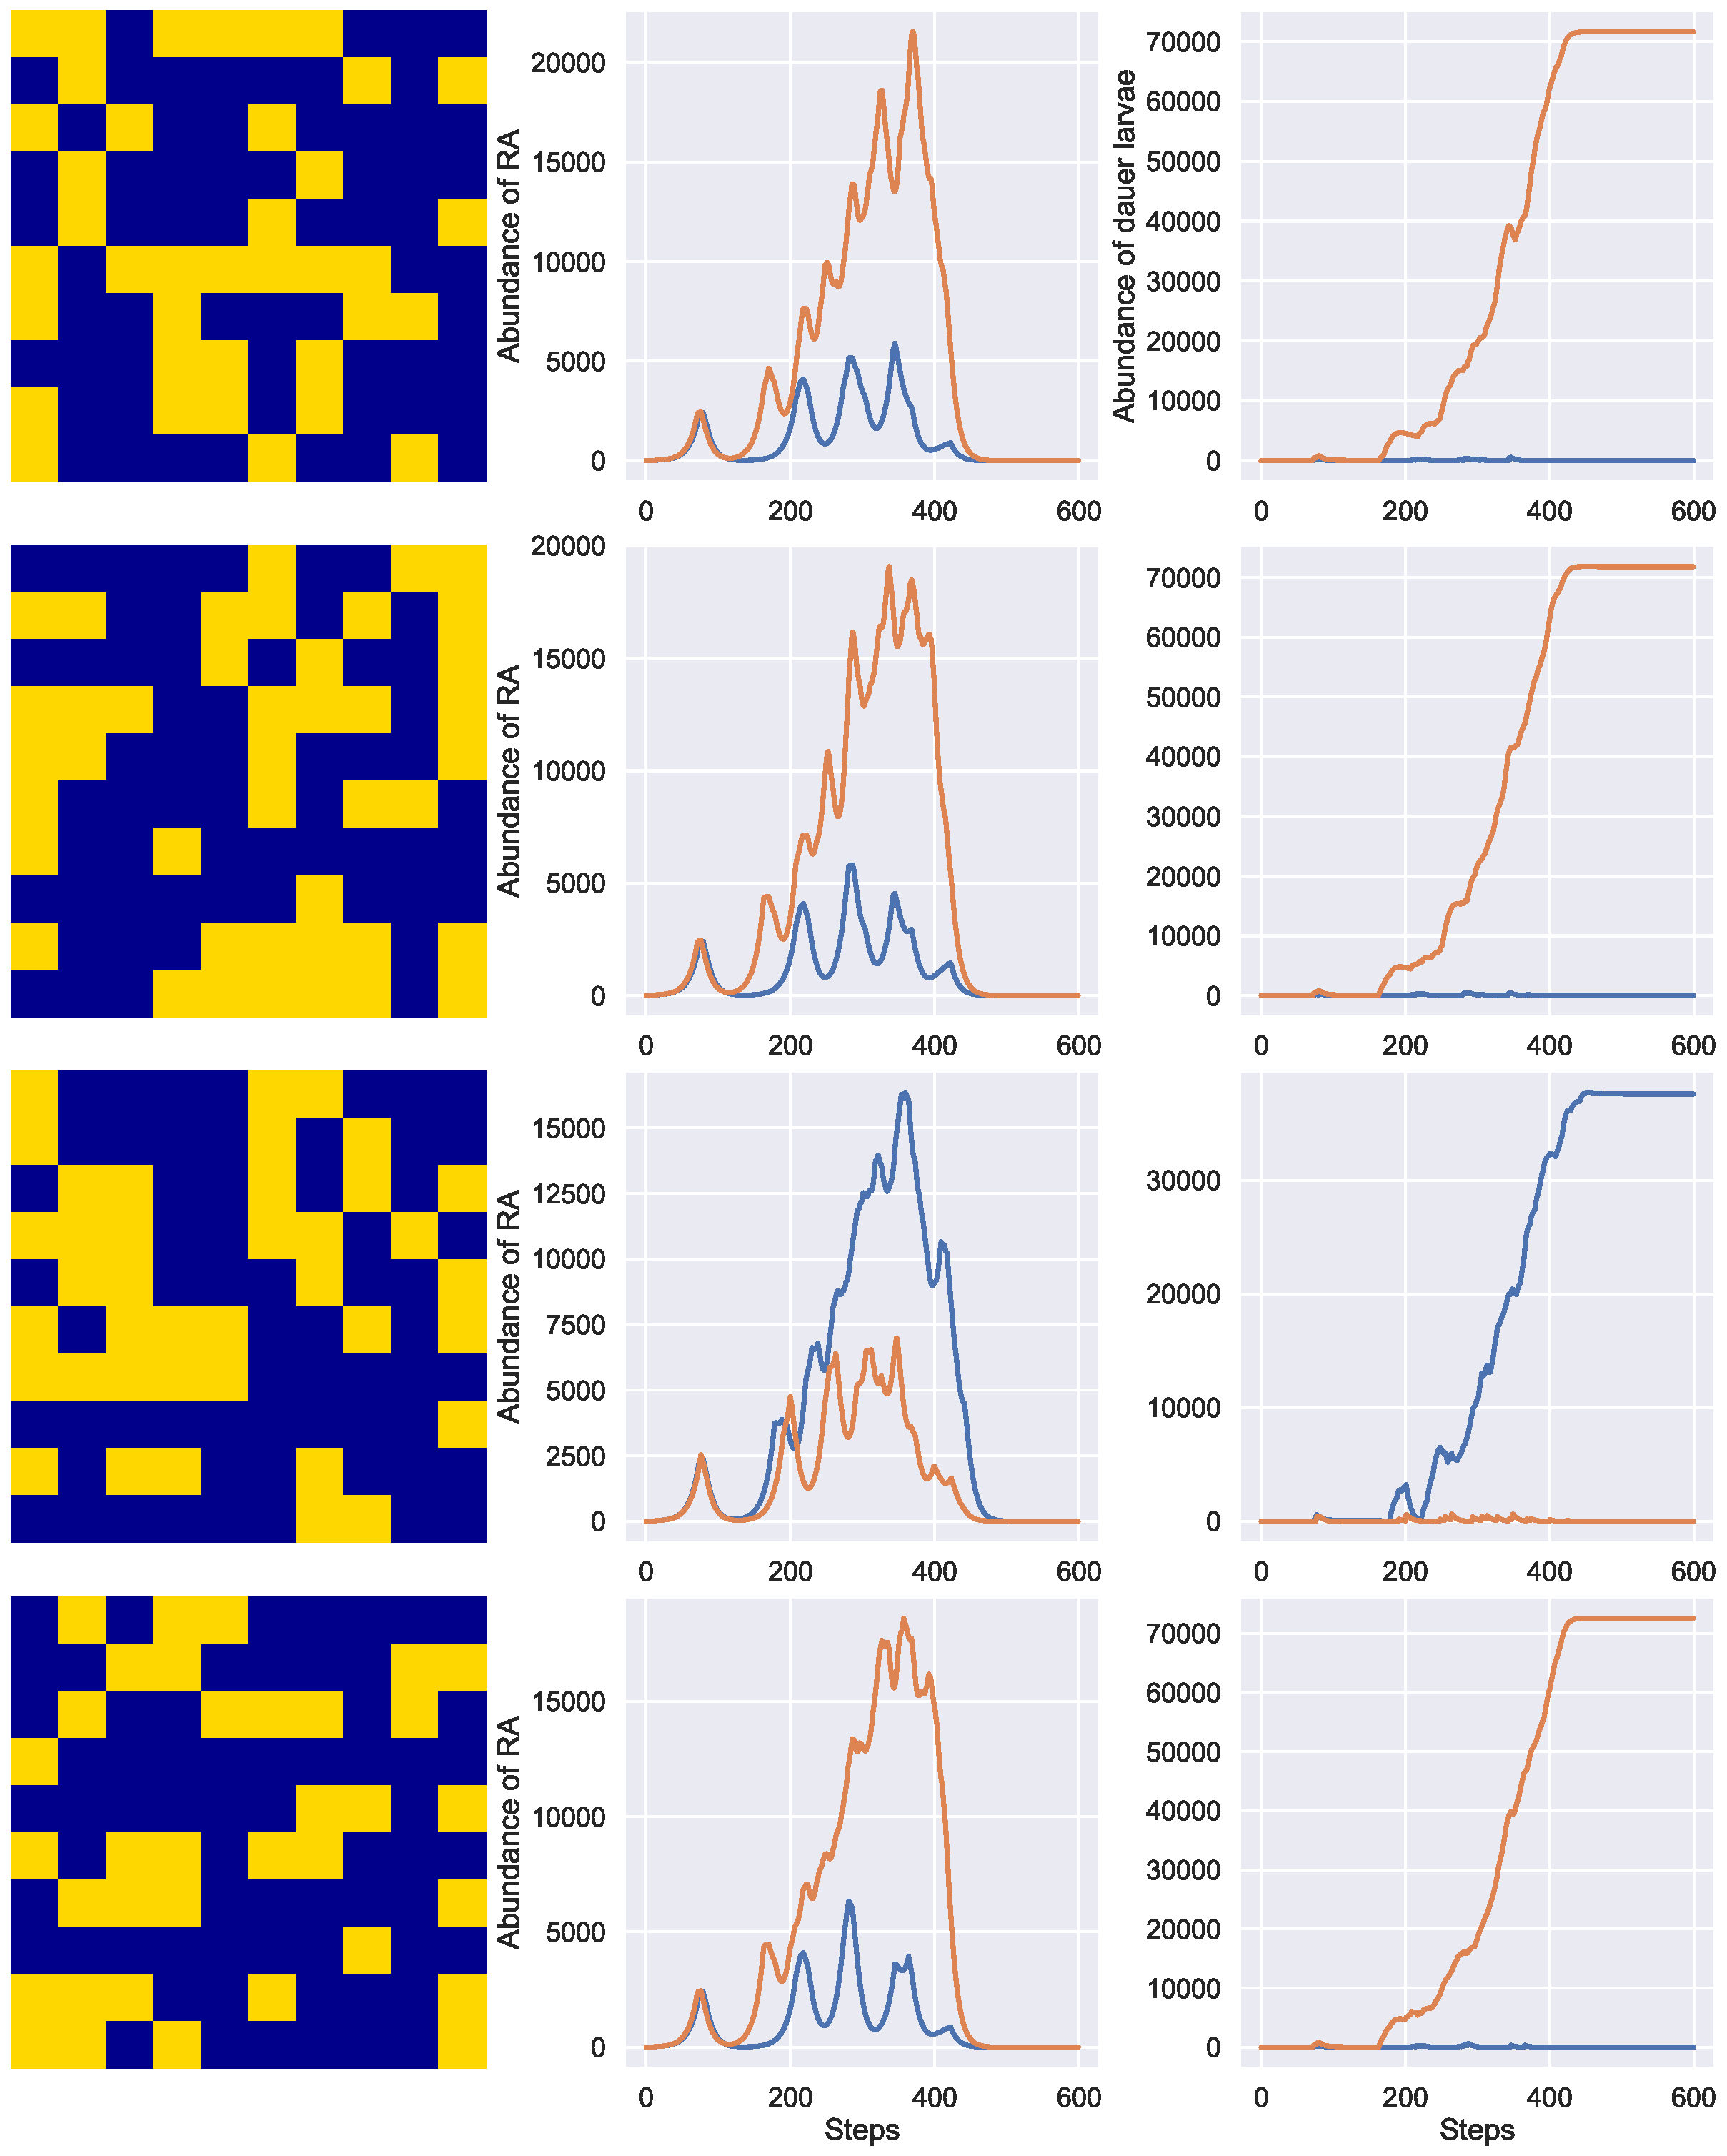
\includegraphics[width=.98\textwidth]{../meta_rand_samples.pdf}};


% %labels
\draw (-6.5, 7.8) node{{\Huge\sf\textbf{a}}};

\draw (-6.5, 4) node{{\Huge\sf\textbf{b}}};

\draw (-6.5, 0) node{{\Huge\sf\textbf{c}}};

\draw (-6.5, -3.5) node{{\Huge\sf\textbf{d}}};


\node at (1.1+1,8.6-16.8) [draw=none, rectangle, fill=darkblue,rotate=0] (g1) {};

\node at (1.1+1, 8.2-16.8) [draw=none, rectangle, fill=gold,rotate=0] (g2) {};

\node at (2.2+1,8.6-16.8) [draw=none, rectangle, fill=none,rotate=0] (g1) {\sf \small \emph{E. coli} OP50};

\node at (3.1+1,8.2-16.8) [draw=none, rectangle, fill=none, rotate=0] (g1) {\sf \small \emph{Novosphingobium} sp. L76};



\end{tikzpicture}


\end{document}